Using just variance and cross channel correlation as features, the SVM performed surprisingly well.  The method achieved 64\% rocAUC on Kaggle and achieved a local prediction accuracy of 89.8\% with a well calibrated threshold.  All local prediction accuracy results are reported using 20 fold cross-validation with a random 20\% section of the data withheld for testing purposes in each fold.  As expected the addition of maximal cross correlation improved the specificity and overall performance of our classification.  This improvement is visualized in Figure \ref{fig:mixedROC}.  The figure shows that maximal cross correlation rises faster and remains higher than that of the simpler variance and covariance dependent methods.  These results suggest that accounting for the temporal effects of the spatial distribution of electrodes captures additional identifying information.  The resulting rocAUC score on Kaggle was found to be 68\% for this method and the local prediction accuracy was found to be 92.6\% with a well calibrated threshold.  The results on Kaggle were significantly lower than any of my cross-validation scores, this is likely due to the fact that the Kaggle challenge withheld 40\% of the data for testing purposes.  Furthermore, the testing data consisted of 50\% preictal segments a much higher percentage than what the training data contained.

\begin{figure}[!t]
\centering
  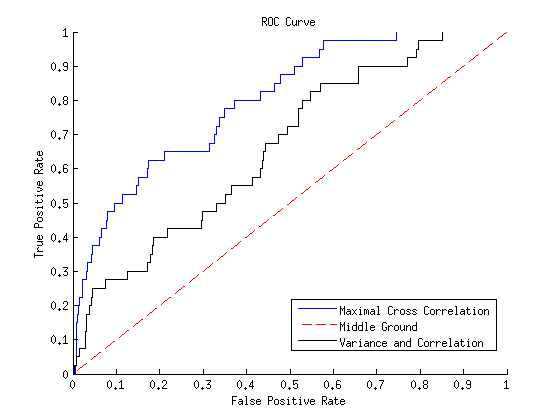
\includegraphics[width=0.48\textwidth]{MixedROC}
  \caption{A graph of the ROC curves for correlation and variance compared against that of maximal cross correlation} \label{fig:mixedROC}
\end{figure}

When looking at the resulting $STL_{max}$ graphs for an interictal and preictal segment, in Figure \ref{fig:STLMax}, there is an immediate disparity between the two.  This suggests that there may be some value to this feature that will confer some ability to distinguish the two classes. However, neither of the graphs seems to really resemble the pattern shown in Figure \ref{fig:origSTLMax} from the work of \cite{iasemidis05}.  The values during the preictal segment are not strictly lower than those during the interictal segment.  Furthermore, the values of the preictal segment do not approximate a strictly decreasing function, in fact quite the opposite.  One hypothesis to explain part of this difference is that the interictal and preictal segments in our work are not taken from closely spaced time points.  In fact, they must be at a minimum a week apart and are likely even much farther apart compared to \cite{iasemidis05} where they seizure events are only about 150 minutes apart.  The non-stationarity of EEG over time could be responsible for some of this difference. 

Despite the differences in appearance of $STL_{max}$, our algorithm accuracy improved to 72\% aucROC on Kaggle when incorporating the additional features.  Due to time constraints, and cluster allocation limits being reach, no graphics are currently available for the $STL_{max}$ algorithm.

\begin{figure}[!t]
\centering
  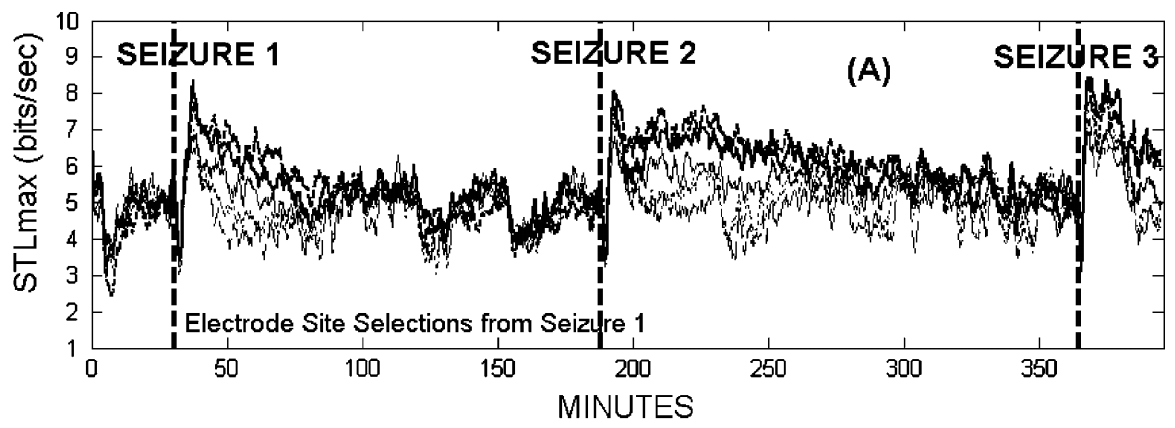
\includegraphics[width=0.48\textwidth]{origSTLMax}
  \caption{Plot of the $STL_{max}$ values as calculated by \cite{iasemidis05} for a series of three seizures} \label{fig:origSTLMax}
\end{figure}

\begin{figure}[!t]
  \centering{
    \subfloat[Interictal]{
      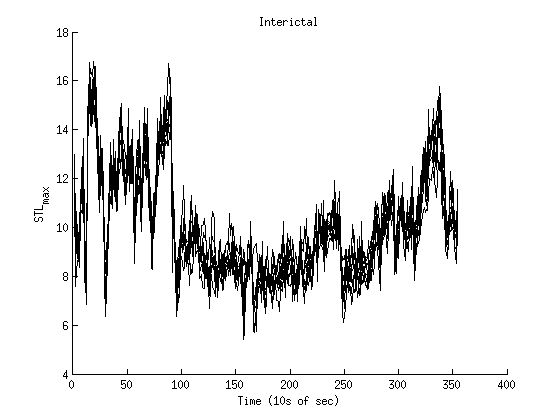
\includegraphics[width=0.3\textwidth]{interictal}%
      \label{fig:interictal}}
    \hfil
    \subfloat[Preictal]{
      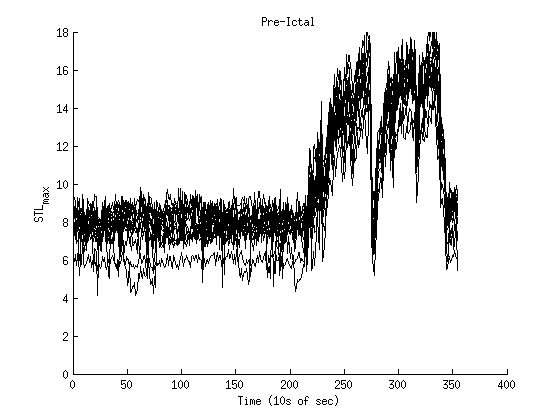
\includegraphics[width=0.3\textwidth]{preictal}%
      \label{fig:preictal}}
  }
  \caption{STLmax For two different 1hr segments of EEG} \label{fig:STLMax}
\end{figure}
